Nykyisen järjestelmän suurin ongelma on sen laajennettavuuden vaikeus. Jos Sikteerin lisäksi halutaan kehittää muita käyttäjien tunnistusta vaativia, joudutaan niihin tekemään käyttäjän tunnistaminen Sikteerin tavoin. Eräs suunnitteilla oleva palvelu on käyttäjien palvelunhallinta, jota kautta jäsenet voisivat lisätä itselleen jäsenmaksuun kuuluvia palveluita, kuten sähköpostialiaksia ja domaineja. Jäsenet kirjautuvat palveluhallintaan henkilökohtaisella Kapsi ry:n käyttäjätunnuksella.

Nykyisessä arkkitehtuurissa järjestelmän sisälle syntyy jälleen uusi paikallinen tietokanta, johon on tallennettu käyttäjän salasana. Keskitetyn tunnistautumispalvelun avulla uusia palveluita voidaan liittää järjestelmään ilman salasanojen kopiointia. Jotta Sikteerin ulkopuolisten web-palveluiden kehittäminen on mahdollista helposti, täytyy erillisillä palveluilla olla tapa tunnistaa käyttäjä uuden palvelun ulkopuolisessa tunnistautumispalvelussa.

Tietojen synkronointi on ongelma myös nykyisessä arkkitehtuurissa, vaikka siihen ei lisättäisi yhtään uutta palvelua. Varsinainen käyttäjähallinta on Sikteerin ulkopuolisessa LDAP-tie\-to\-kan\-nas\-sa, josta data synkronoidaan Sikteerin omaan tietokantaan. Käyttäjän tietoihin tallennettujen tunnistetietojen perusteella Sikteeri tunnistaa käyttäjät. Tulevaisuudessa tietojen synkronointia ei haluta tehdä, vaan käyttäjien tunnistetiedot halutaan säilyttää vain LDAP-tietokannassa. Koska käyttäjätietokantaan on tallennettu henkilökohtaista dataa, kuten henkilötunnuksia, halutaan integroinnit siihen pitää mahdollisimman vähälukuisina.

Kuvassa \ref{kapsi_nykyinen_uusi} on nykyisten hallintatyökalujen arkkitehtuuri, kun siihen on lisätty keskitetty tunnistautumispalvelu. Tunnistautumispalvelu on ainoa komponentti, jolla on pääsy LDAP-tietokantaan. Sikteerin tietokannassa säilytetään vain listaa käyttäjätunnuksista, joilla on oikeus käyttää järjestelmää. Kaikki muut käyttäjään liittyvät tiedot ovat vain LDAP:ssa ja ne haetaan sieltä tarvittaessa tunnistautumispalvelun kautta.

\begin{figure}[ht]
\centering
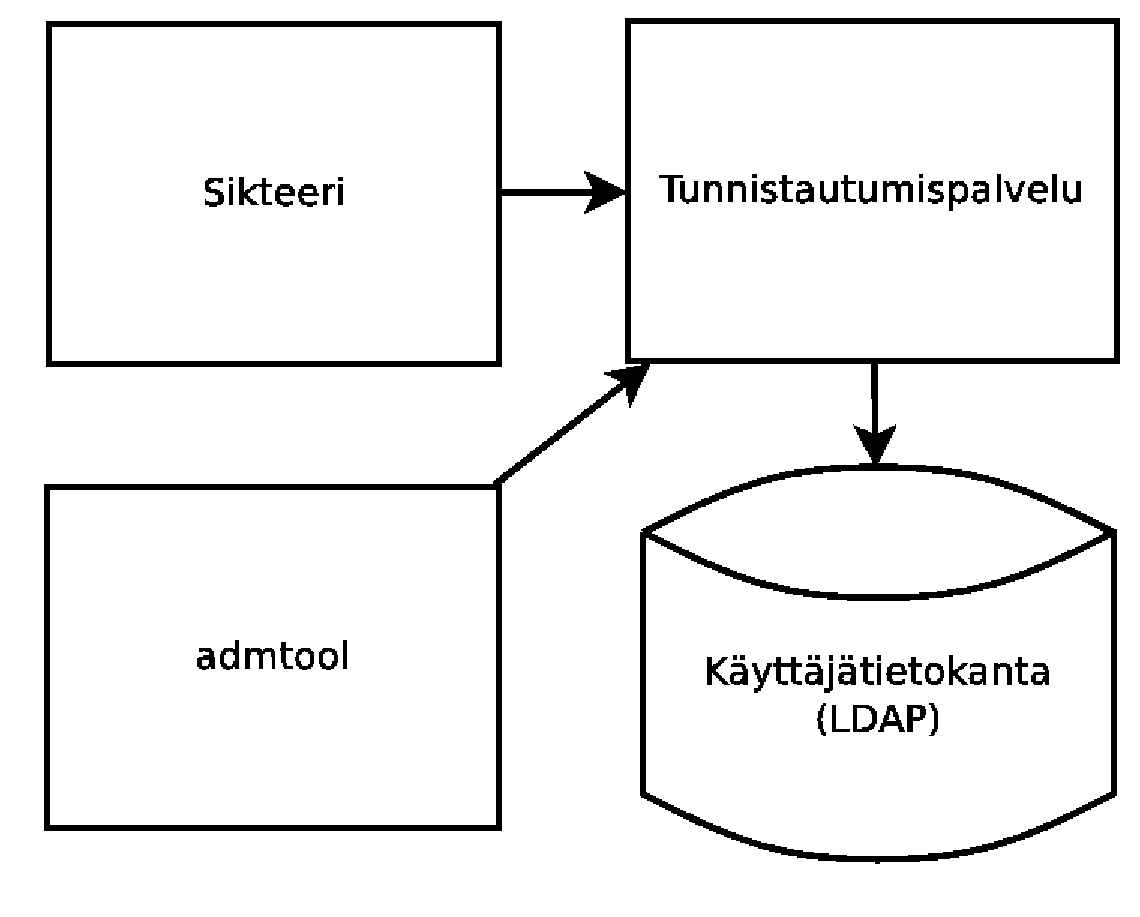
\includegraphics[width=.6\textwidth]{toteutus/muutostarve/kapsi_uusi.eps}
\caption{Keskitettyä tunnistautumispalvelua käyttävä hallintatyökalujen arkkitehtuuri.}%
\label{kapsi_nykyinen_uusi}
\end{figure}

Sikteeri on vuosien varrella paisunut yleiseksi toiminnanohjausjärjestelmäksi, jonka arkkitehtuuria kehittäjät haluaisivat viedä palvelusuuntautuneiden arkkitehtuurien suuntaan. Tällöin esimerkiksi laskutukseen tai jäsenrekisteriin liittyvät tehtävät voitaisiin toteuttaa omana palveluna. Kuvassa \ref{kapsi_uusi} on esitetty tavoiteltu arkkitehtuuri, jossa Sikteerin laskutus- ja jäsenrekisteripalvelut ovat itsenäisiä web-sovelluksia ja joiden rinnalla on admtool-komentorivityökalu sekä käyttäjien palvelunhallinta. Seuraavassa luvussa esiteltävän arkkitehtuurin puitteissa ei oteta kantaa Sikteerin palvelusuuntautuneeseen arkkitehtuuriin, vaan pyritään löytämään ratkaisu, joka mahdollistaa myös ko. arkkitehtuurimuutoksen tulevaisuudessa.

\begin{figure}[ht]
\centering
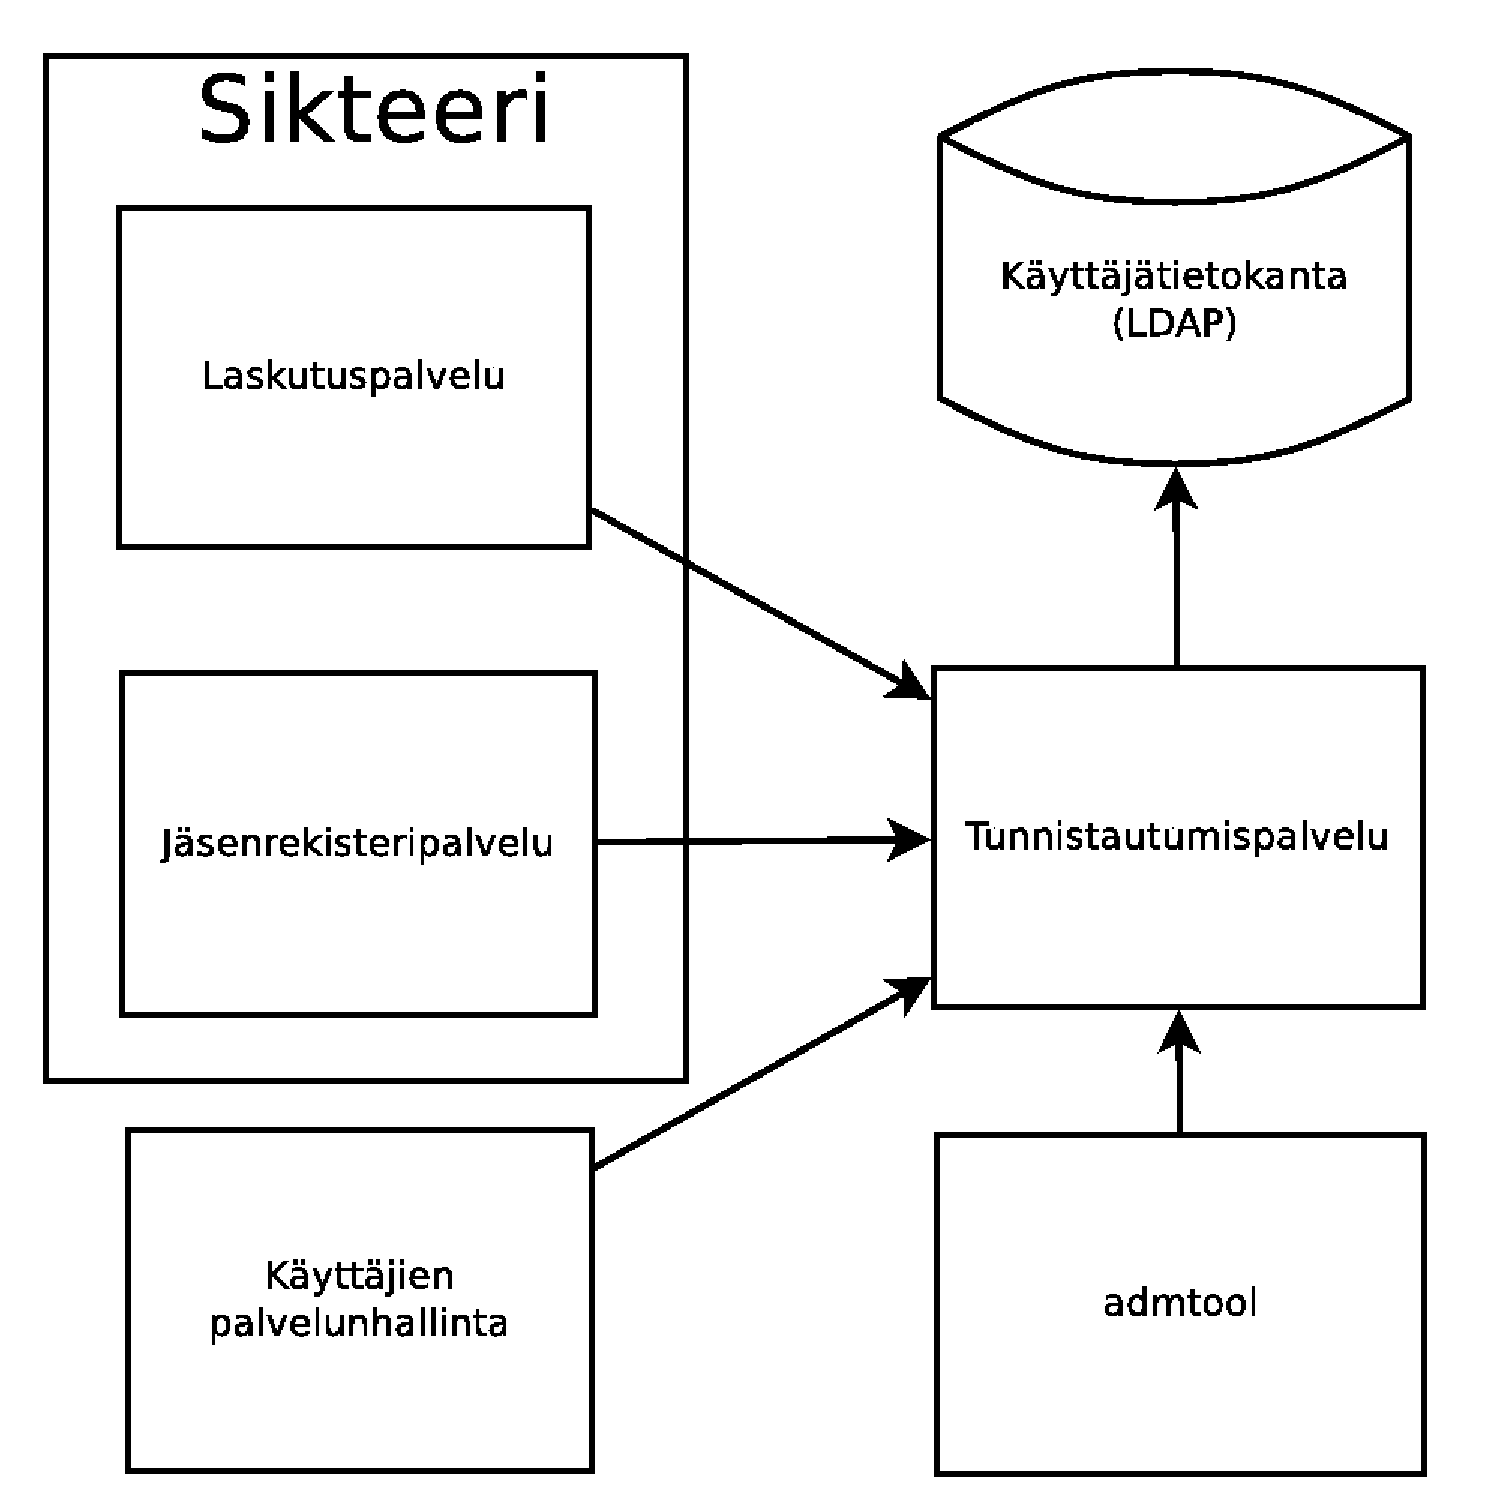
\includegraphics[width=.6\textwidth]{toteutus/muutostarve/kapsi_uusi_soa.eps}
\caption{Palvelusuuntautuneiden arkkitehtuurien mukainen kuvaus Kapsin järjestelmästä. Sikteerin palvelut on jaoteltu omiksi komponenteiksi ja järjestelmään on lisätty keskitetty tunnistautumispalvelu.}%
\label{kapsi_uusi}
\end{figure}